\section{Evaluation}\label{sec:evaluation}

In this section, we evaluate the advancements presented in \cref{sec:searchspace_construction} to determine their performance and scalability impact using a case study with various applications. 
First, we discuss how we compare against the current state-of-the-art solvers in \cref{subsec:evaluation_compared_frameworks}.
% First, we discuss the way current state-of-the-art solvers are used to compare against in \cref{subsec:evaluation_compared_frameworks}. 
Following this, we evaluate the solvers on a collection of synthetically generated search spaces to assess scalability differences between solvers under various search space characteristics in \cref{subsec:evaluation_synthetic}. 
Finally, we evaluate the solvers on a variety of real-world applications to indicate actual performance in \cref{subsec:evaluation_real-world}. 

% \Cref{sec:searchspace_construction} proposed a new approach and several optimizations to the search space construction. 
% To assess the performance of this new approach, synthetic and real-world tests are performed, to assess scaling differences under various characteristics and to indicate real-world performance, respectively. 

The evaluations in this work are performed on the sixth generation DAS \href{https://www.cs.vu.nl/das/clusters.shtml}{VU-cluster}~\cite{DASMediumScaleDistributedSystem} using an NVIDIA A4000 GPU node. The GPU is paired with a 24-core AMD EPYC-2 7402P CPU, 128 GB of memory, and running Rocky Linux 4.18. While none of the tested solvers use the GPU, we use a GPU node to obtain an environment as similar as possible to real-world GPU auto-tuning. 
For all tests performed, the results of each solver were validated against a brute-forced solution of the search space. 

% \subsection{Experimental Setup} \label{subsec:evaluation_setup}
% To assess the feasibility of tuning large search spaces with Kernel Tuner, this evaluation is performed on four applications with large search spaces. 
% The selected kernels are the top-three kernels by search space size in the Benchmark suite for Auto-Tuners (BAT) \cite{BenchmarkingSuiteKerneltuners}. These are \textit{Dedispersion}, \textit{Hotspot}, \textit{ExpDist}. In addition, we use the search space of the \textit{MicroHH} computational fluid dynamics kernel \cite{MicroHH2017}. The characteristics of these search spaces are seen in \Cref{tab:searchspaces_real_world_overview}. 

% \begin{table}[tbh]
%     \centering
%     \small
%     \begin{tabularx}{\linewidth}{|X|X|X|X|}
%         \hline
%         \textbf{Name} & \textbf{Cartesian size} & \textbf{Dimensions} & \textbf{Restrictions} \\
%         \hline
%         Dedispersion & 22272 & 8 & 3 \\\hline
%         Expdist & 9732096 & 10 & 4 \\\hline
%         Hotspot & 22200000 & 11 & 5 \\\hline
%         Microhh & 1166400 & 13 & 8 \\
%         \hline
%     \end{tabularx}
%     \caption{Overview of the characteristics of the search spaces evaluated on.}
%     \label{tab:searchspaces_real_world_overview}
% \end{table}

\subsection{Comparison against state-of-the-art} \label{subsec:evaluation_compared_frameworks}
To provide additional reference on the performance in this evaluation, we compare the results to the state-of-the-art in auto-tuning search space construction: Auto-Tuning Framework (ATF) \cite{raschATFGenericAutoTuning2017}, which specifically focuses on large optimization spaces with interdependent parameters. 
ATF has two independent implementations, in C++ and Python, both of which we use in this evaluation to compare our method to. The C++ version available as of August 2024 with Python bindings is used and denoted as \textit{ATF} in the results. The Python version, called \textit{pyATF}, is used at version 0.0.9, the latest version at the time of writing.

For the majority of the discussed solvers, the notation of tunable parameters and constraints is largely separated (e.g. a user first defines the tunable parameters and values, then defines the constraints to apply). However, both implementations of ATF have a notation that combines the definition of tunable parameters, values, and constraints into one statement. As a result of this, constraints can only reference tunable parameters that have been previously defined. Due to the large number of search spaces used in this evaluation, it is not feasible to write each of these search space definition files by hand for both ATF implementations, and we have instead written parsers that define the ATF search space files from an abstract definition of the search spaces. These parsers take the aforementioned parameter-constraint order relation into account and convert to built-in ATF types such as intervals where applicable to provide search space definitions that are as closely possible to what is expected by the authors. 
To reflect the user experience as accurately as possible, the search space file compilation time is included in the total construction time. 
The C++ version of ATF and search space files is compiled with GCC 9.4.0 using the optimization commands recommended by the ATF documentation. 

In addition, we compare against PySMT at version 0.9.6 using the Microsoft Z3 solver to evaluate differences in scalability for solvers without support for resolving all solutions, as described in \cref{subsec:searchspace_construction_packages}. The Z3 theorem prover is developed by Microsoft for software verification and analysis \cite{Z3solver}, and is the winner of the 3rd Annual Satisfiability Modulo Theories Competition (SMT-COMP)~\cite{smtcomp2007}. 
Similarly to ATF, we have written a parser to use PySMT-specific operations where applicable. 

\ifdoubleblind
We have published the implementation of this evaluation in a repository for further reference.
\else
We have published the implementation of this evaluation in a repository\footnote{\href{https://github.com/fjwillemsen/kernel_tuner_paper}} for further reference.
\fi

\subsection{Synthetic Tests} \label{subsec:evaluation_synthetic}
To understand how search space characteristics influence the construction time of the evaluated solvers, we use synthetic tests. 
We have generated a set of search spaces with a varying number of dimensions (between 2 and 5), target Cartesian sizes (with $\{1\times 10^{4}, 2\times 10^{4}, 5\times 10^{4}, 1\times 10^{5}, 2\times 10^{5}, 5\times 10^{5}, 1\times 10^{6}\}$), and number of constraints (between 1 and 6). While these arbitrary parameters result in search spaces that are not as large and do not have as many tunable parameters as the real-world search spaces evaluated on in \cref{subsec:evaluation_real-world}, the goal of these in total 112 synthetic search spaces is to gain insight into which of these factors has the greatest effect on performance, and which solution provides good scalability across the variations in these factors.
% $\{10000, 20000, 50000, 100000, 200000, 500000, 1000000\}$

\begin{figure}[!htb]
    \centering
    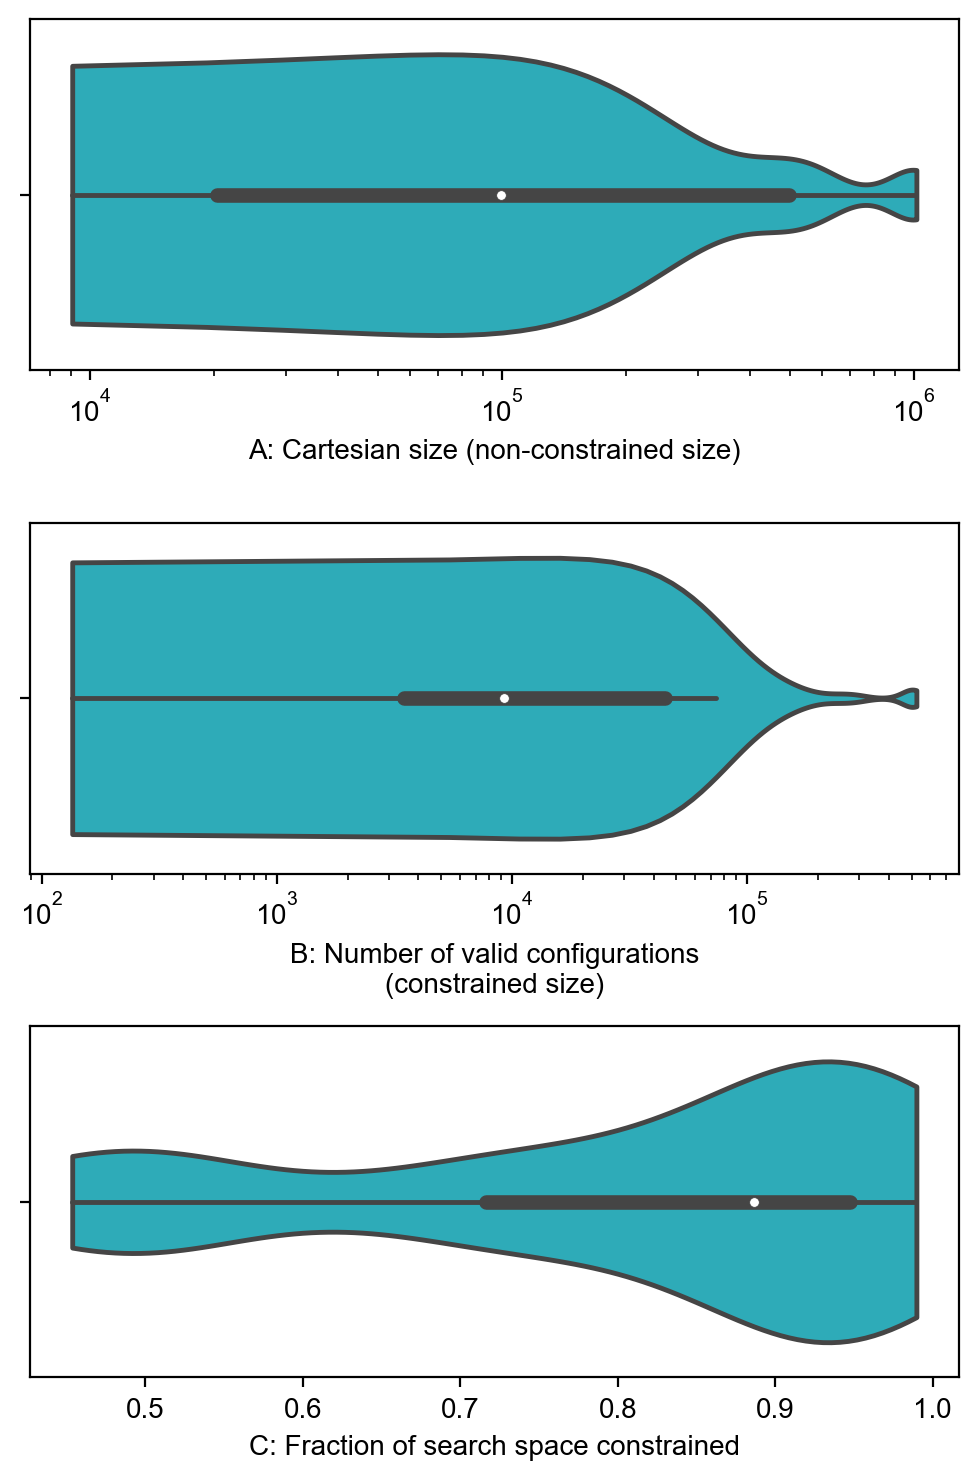
\includegraphics[width=0.95\linewidth]{ics25template/figures/searchspace_construction/results_synthetic_violin.png}
    \caption{Characteristics of the 112 synthetic search spaces}
    \Description[Characteristics of the 112 synthetic search spaces]{Characteristics of the 112 synthetic search spaces}
    \label{fig:searchspaces_synthetic_characteristics}
\end{figure}

\begin{figure*}[!htb]
    \centering
    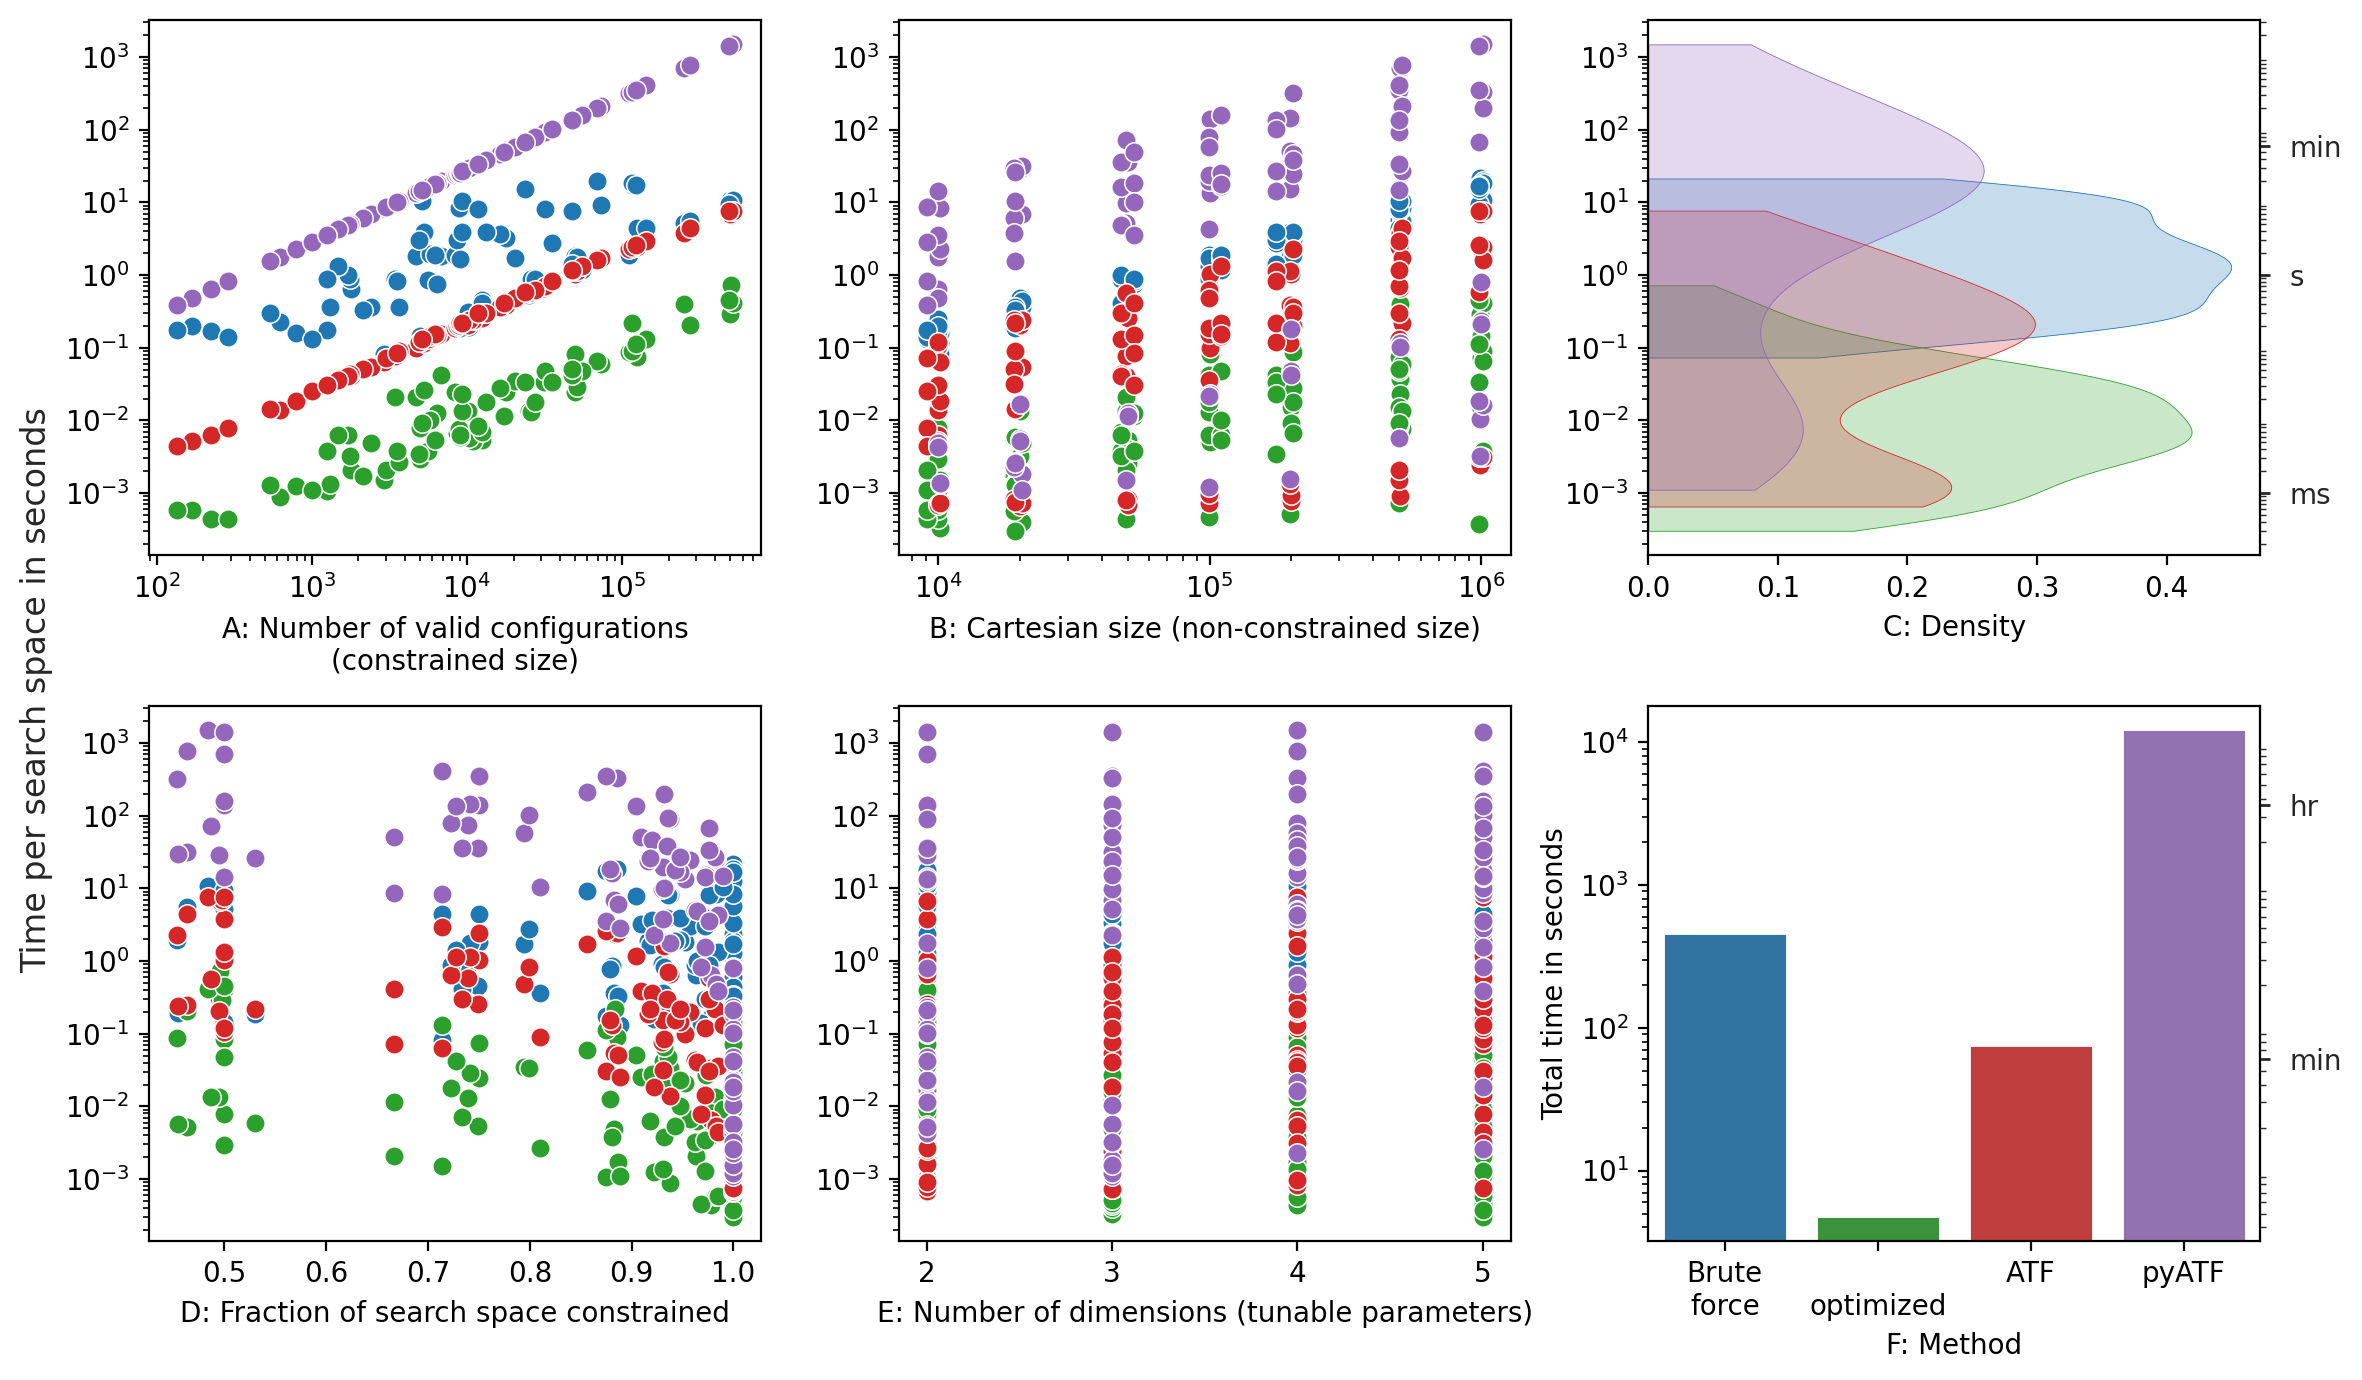
\includegraphics[width=1.0\textwidth]{ics25template/figures/searchspace_construction/results_synthetic.png}
    \caption{Search space construction performance on synthetic tests. Lower times are better. Colors correspond to \Cref{fig:results_synthetic}F barplot methods.}
    \Description[search space construction performance]{search space construction performance on synthetic tests. Lower times are better.}
    \label{fig:results_synthetic}
\end{figure*}

Given a Cartesian size, a number of dimensions, and a number of constraints, we want to generate a synthetic search space. 
To prevent an unfair advantage to solvers optimized for a limited number of dominant dimensions, this number of values per dimension $v$ is kept approximately uniform. 
This is done by first determining the number of values per dimension as $v = s^{\frac{1}{d}}$, where $s$ is the desired Cartesian size and $d$ is the desired number of dimensions. 
For each of the dimensions, a linear space with $v$ number of elements is instantiated. 
Given a non-integer value of $v$, this is rounded to an integer for all but the last dimension, where $v$ is rounded contradictory (e.g. $5.8 \rightarrow 5$, $5.2 \rightarrow 6$) to be closer to the desired Cartesian size. 
A list of constraints involving a variety of operations is generated for each combination of dimensions, which are randomly chosen up to the desired number of constraints. 

\Cref{fig:searchspaces_synthetic_characteristics} shows the dispersion of the resulting 112 search spaces in violin plots for three characteristics: the Cartesian size, the number of valid configurations, and the fraction of the search space constrained (the number of valid configurations relative to the total Cartesian size). 
As the application of the constraints does not affect the already uniformly distributed number of parameters, this characteristic is not included in the figure. 
These violin plots should be interpreted by examining both the y-axis width and central tendencies of the distributions. The wider sections indicate a higher density of search spaces with the associated x-axis values, while the white dot represents the median, and the thick bar around it marks the interquartile range.
\Cref{fig:searchspaces_synthetic_characteristics}A shows the actual Cartesian size, representing the total number of possible configurations before constraints are applied, revealed to be in line with the set of target values used. 
\Cref{fig:searchspaces_synthetic_characteristics}B depicts the number of valid configurations remaining after constraints are enforced, which follows a distribution similar to the Cartesian size of \Cref{fig:searchspaces_synthetic_characteristics}A, yet covering a wider range on the lower end, also demonstrating the general effect of constraints on the difference between the Cartesian size and actual number of configurations. 
Finally, \Cref{fig:searchspaces_synthetic_characteristics}C displays the fraction of sparsity of the search space, i.e. the fraction of non-valid configurations relative to the Cartesian size. 
Though the fraction of constrained configurations is skewed toward higher values, indicating a propensity towards sparsity, a wide range of variations in sparsity is present. 


The performance on the synthetic search spaces is displayed in various plots in \Cref{fig:results_synthetic}, where the colors used correspond to the colors of the methods in the \Cref{fig:results_synthetic}F barplot. 

It is noteworthy how in \cref{fig:results_synthetic}A there appears to be an approximately linear correlation between the time required to construct a search space and the number of valid configurations, which is not as evident in the other characteristics in \cref{fig:results_synthetic}B, \cref{fig:results_synthetic}D, and \cref{fig:results_synthetic}E. 
% Furthermore, \cref{fig:results_synthetic}A illustrates the relationship between the number of valid configurations (constrained size) and the time required to construct the search space. 
Our \textit{optimized} solver consistently achieves the lowest execution times, with several orders of magnitude better performance compared to the \textit{brute force}, \textit{ATF}, and \textit{pyATF} solvers. The \textit{pyATF} solver exhibits the highest execution times, being generally outperformed even by brute-force solving, an interesting result which we will examine using the other characteristics. 

\cref{fig:results_synthetic}B examines the effect of the Cartesian size on execution time, where a general trend of increasing computation time with larger Cartesian sizes can be seen. Interestingly, the \textit{ATF} and \textit{pyATF} solvers in some cases do not conform to this trend, creating a large variance in their performances.

The reason for this appears to be found in \cref{fig:results_synthetic}D, which shows the relationship between the fraction of the sparsity of a search space and execution time. Both \textit{ATF} and \textit{pyATF} appear to be severely optimized for very sparse search spaces, in contrast to the other methods. 

\Cref{fig:results_synthetic}C presents the execution time distributions of the solvers as a continuous probability density curve using a kernel density estimate (KDE). Particularly noteworthy is the bimodality demonstrated by \textit{ATF} and \textit{pyATF}, which appears to be caused by the sensitivity to search space sparsity seen in \cref{fig:results_synthetic}D.

Observing \cref{fig:results_synthetic}E, it appears that there is no strong correlation between solver performance and the number of tunable parameters. 

\Cref{fig:results_synthetic}F summarizes the overall performance of each solver in a bar chart.
It is remarkable that pyATF takes considerably longer than the brute-force method on these search spaces, which might be due to how optimized the ATF approach is to highly sparse search spaces.
Our optimized method achieves a 96x speedup over the brute-force method (4.75 seconds versus 455.3 seconds), a 16x speedup over ATF, and a 2547x speedup over pyATF. 
% Total speedup of method 'optimized' (4.75 seconds) over 'Bruteforce' (455.29 seconds): 95.9x
% Total speedup of method 'ATF' (74.08 seconds) over 'Bruteforce' (455.29 seconds): 6.1x
% Total speedup of method 'pyATF' (12098.64 seconds) over 'Bruteforce' (455.29 seconds): 0.0x

% The performance on the synthetic search spaces is seen in \Cref{fig:results_synthetic}, where the colors used correspond to the colors of the methods in the \Cref{fig:results_synthetic}F barplot. In \Cref{fig:results_synthetic}, it can be seen that the duration is generally more influenced by the total size of the search space (in particular the constrained size of \cref{fig:results_synthetic}A) than the ratio of valid to non-valid configurations (\cref{fig:results_synthetic}D) or the number of dimensions (\cref{fig:results_synthetic}E). \Cref{fig:results_synthetic}F shows the overall performance difference, indicating that the optimized method achieves a 96x speedup over the brute-force method (4.75 seconds versus 455.3 seconds). 
% In contrast, pyATF takes considerably longer than the brute force method on these search spaces. % Both pyATF and ATF appear to scale linearly with the number of valid configurations. 
% It is noteworthy that the C++ version of ATF comes somewhat close to the performance of our optimized method, but only when nearly all of the search space is constrained, as seen in \cref{fig:results_synthetic}D. 
% Both the ATF and pyATF density distributions interestingly demonstrate bimodality in the top plot of \cref{fig:results_synthetic}C, which intersects with the performance difference of both implementations over the fraction of search space constrained in \cref{fig:results_synthetic}D, confirming that the ATF approach is heavily optimized for very sparse search spaces.
% In general, our new method is $\sim$96x faster than brute force, $\sim$15x faster than ATF, and $\sim$2547x faster than pyATF on these synthetic search spaces. 
% % Synthetic: 
% % Total speedup of method 'Old' (675.44 seconds) over 'Bruteforce' (455.29 seconds): 0.7x
% % Total speedup of method 'New' (4.75 seconds) over 'Bruteforce' (455.29 seconds): 95.9x
% % Total speedup of method 'ATF' (74.08 seconds) over 'Bruteforce' (455.29 seconds): 6.1x
% % Total speedup of method 'pyATF' (12098.64 seconds) over 'Bruteforce' (455.29 seconds): 0.0x
% % Real-world: 
% % Total speedup of method 'Old' (8347.66 seconds) over 'Bruteforce' (65197.71 seconds): 7.8x
% % Total speedup of method 'New' (2.88 seconds) over 'Bruteforce' (65197.71 seconds): 22668.4x
% % Total speedup of method 'ATF' (135.3 seconds) over 'Bruteforce' (65197.71 seconds): 481.9x
% % Total speedup of method 'pyATF' (2474.65 seconds) over 'Bruteforce' (65197.71 seconds): 26.3x

\begin{figure}[!htb]
    \centering
    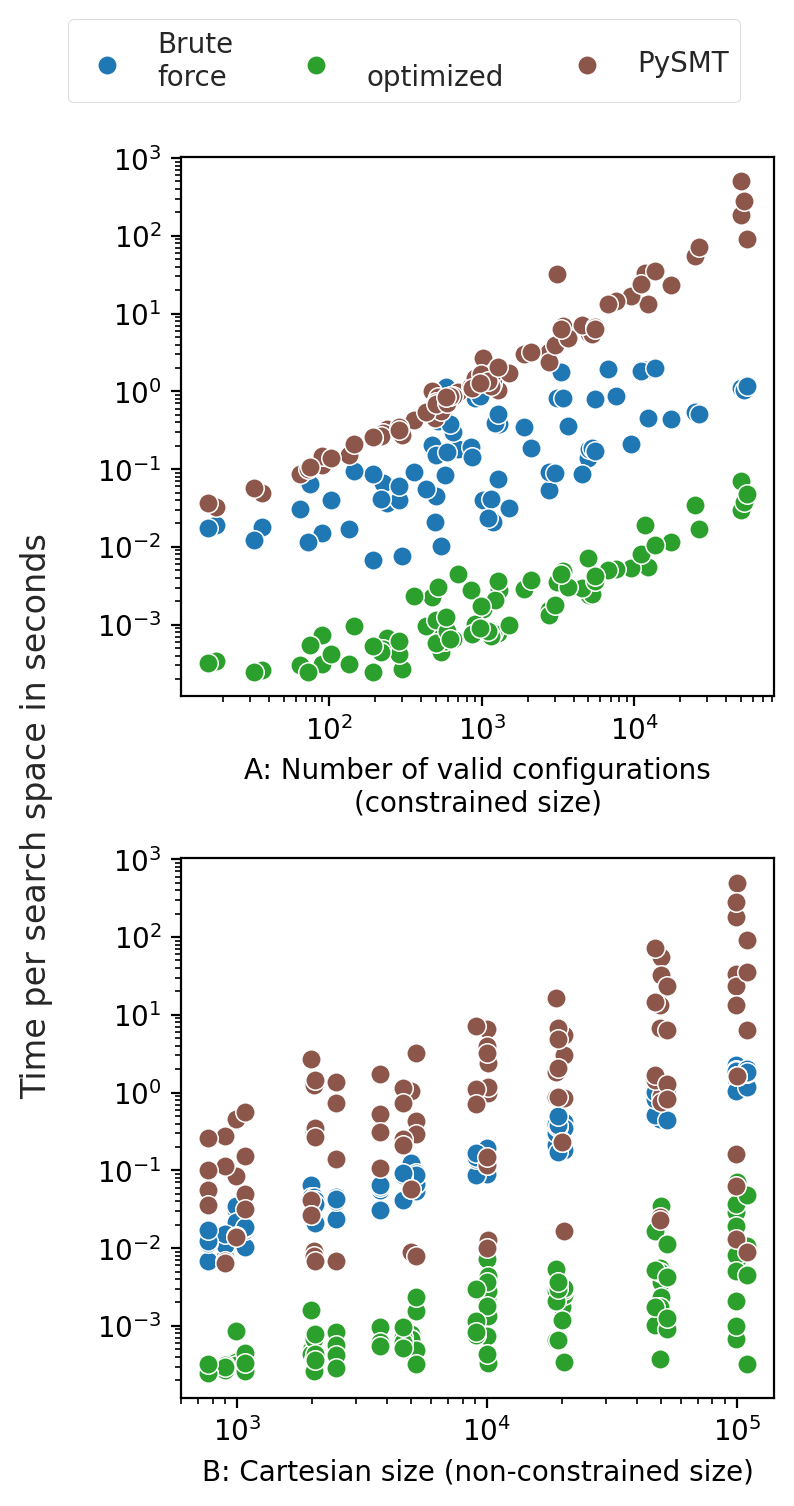
\includegraphics[width=0.95\linewidth]{ics25template/figures/searchspace_construction/results_synthetic_pysmt_100000.png}
    \caption{Search space construction performance of PySMT on synthetic tests (reduced search spaces size).}
    \Description[search space construction performance synthetic with PySMT]{search space construction performance on synthetic tests, including PySMT.}
    \label{fig:results_synthetic_pysmt}
\end{figure}

As described in \cref{subsec:searchspace_construction_packages}, a traditional solver without support for finding all solutions requires adding the previous solution as a constraint and iterating over the solutions until all solutions have been found. To demonstrate the lack of scalability of such a solver, \cref{fig:results_synthetic_pysmt} compares PySMT using the Microsoft Z3 solver to the brute-force method and the optimized solver. 
To make executing this experiment feasible, we had to reduce the size of the generated synthetic search spaces by one order of magnitude in this instance. 
As seen in \cref{fig:results_synthetic_pysmt}, PySMT performs poorly relative to both brute force and our optimized method. As expected, this difference increases as the number of valid configurations increases, demonstrating the infeasibility of this approach when many valid configurations are present. 
Despite the reduced search space sizes, PySMT with the Z3 solver still takes nearly a thousand seconds on the largest search spaces, whereas the brute-force solver takes about ten seconds. 
Our optimized solver takes about as long to solve the largest search spaces as PySMT with the Z3 solver takes to solve the smallest search spaces. PySMT with the Z3 solver will not be included in the remainder of the evaluation as it is infeasible to evaluate the large search spaces of the real-world applications. 

% Total speedup of method 'original' (8353.17 seconds) over 'Brute
% force' (65230.47 seconds): 7.8x
% Total speedup of method '
% optimized' (3.16 seconds) over 'Brute
% force' (65230.47 seconds): 20610.7x
% Total speedup of method 'ATF' (137.83 seconds) over 'Brute
% force' (65230.47 seconds): 473.3x
% Total speedup of method 'pyATF' (2816.74 seconds) over 'Brute
% force' (65230.47 seconds): 23.2x

% old results:
% Total speedup of method 'Old' (6.79 seconds) over 'Bruteforce' (4.55 seconds): 0.7x
% Total speedup of method 'New' (0.07 seconds) over 'Bruteforce' (4.55 seconds): 63.8x
% Total speedup of method 'ATF' (1.07 seconds) over 'Bruteforce' (4.55 seconds): 4.3x
% Total speedup of method 'pyATF' (121.72 seconds) over 'Bruteforce' (4.55 seconds): 0.0x
% Total speedup of method 'PySMT' (88.25 seconds) over 'Bruteforce' (4.55 seconds): 0.1x


\subsection{Real-world Applications} \label{subsec:evaluation_real-world}

\begin{table*}[htb]
    \centering
    \scriptsize
    \begin{tabularx}{\linewidth}{|l|X|X|X|X|X|X|X|X|}
        \hline
        % \textbf{Name} & \textbf{Cartesian size} & \textbf{Constraint size} & \textbf{Number of parameters (dimensions)} & \textbf{Number of constraints} & \textbf{Avg. unique parameters per constraints} & \textbf{Range of number of values per parameter} & \textbf{\% of configurations in Cartesian size}  \\
        % \hline
        % Dedispersion & 22272 & 11130    & 8 & 3     & 2 & 1 - 29 & 49.973 \\\hline
        % ExpDist & 9732096 & 294000      & 10 & 4    & 2 & 1 - 11 & 3.021 \\\hline
        % Hotspot & 22200000 & 349853     & 11 & 5    & 3.8 & 1 - 37 & 1.576 \\\hline
        % GEMM & 663552 & 116928          & 17 & 8    & 3.25 & 1 - 4 & 17.622 \\\hline
        % MicroHH & 1166400 & 138600      & 13 & 8    & 2.375 & 1 - 10 & 11.883 \\\hline
        % ATF PRL 2x2 & 36864 & 1200      & 20 & 14   & 2.429 & 1 - 3 & 3.255 \\\hline
        % ATF PRL 4x4 & 9437184 & 10800   & 20 & 14   & 2.429 & 1 - 4 & 0.114 \\\hline
        % ATF PRL 8x8 & 2415919104 & 48720 & 20 & 14  & 2.429 & 1 - 8 & 0.002 \\\hline
        % \textit{Mean} & \textit{307322534} & \textit{121403} & \textit{14.875} & \textit{8.75}  & \textit{2.589} & \textit{1} - \textit{13.25} & \textit{10.93} \\\hline
        
        \textbf{Name} & \textbf{Cartesian size} & \textbf{Constraint size} & \textbf{Number of parameters (dimensions)} & \textbf{Number of constraints} & \textbf{Avg. unique parameters per constraints} & \textbf{Range of number of values per parameter} & \textbf{\% of configurations in Cartesian size} & \textbf{Avg. number of constraint evaluations required}  \\
        \hline
        Dedispersion & 22272 & 11130    & 8 & 3     & 2 & 1 - 29 & 49.973     & 33414 \\\hline
        ExpDist & 9732096 & 294000      & 10 & 4    & 2 & 1 - 11 & 3.021      & 23889240 \\\hline
        Hotspot & 22200000 & 349853     & 11 & 5    & 3.8 & 1 - 37 & 1.576    & 65900294 \\\hline
        GEMM & 663552 & 116928          & 17 & 8    & 3.25 & 1 - 4 & 17.622   & 2576736 \\\hline
        MicroHH & 1166400 & 138600      & 13 & 8    & 2.375 & 1 - 10 & 11.883 & 4763700 \\\hline
        ATF PRL 2x2 & 36864 & 1200      & 20 & 14   & 2.429 & 1 - 3 & 3.255   & 268680 \\\hline
        ATF PRL 4x4 & 9437184 & 10800   & 20 & 14   & 2.429 & 1 - 4 & 0.114   & 70708680 \\\hline
        ATF PRL 8x8 & 2415919104 & 48720 & 20 & 14  & 2.429 & 1 - 8 & 0.002   & 18119076600 \\\hline
        \hline
        \textit{Mean} & \textit{307322534} & \textit{121403} & \textit{14.875} & \textit{8.75}  & \textit{2.589} & \textit{1} - \textit{13.25} & \textit{10.93} & \textit{2285902168} \\\hline
    \end{tabularx}
    \caption{Overview of the basic characteristics of the real-world search spaces and the mean values for each of the columns.}
    \label{tab:searchspaces_real_world_overview}
\end{table*}
% Avg. unique involved parameters per restriction:
% d = [[2,2,2], [2,2,2,2], [2,2,2,6,7], [2,3,3,3,3,4,4,4], [4,3,2,2,2,2,2,2], [2,2,2,2,3,3,3,2,2,2,3,3,3,2]]    # last entry is the same for all PRL spaces
% for s in d:
%   print(round(sum(s)/len(s), 3))

To evaluate solver performance on the search spaces of real-world applications, we select the three largest search spaces in the Benchmark suite for Auto-Tuners (BAT)~\cite{BenchmarkingSuiteKerneltuners}. 
These are \textit{Dedispersion}, \textit{Hotspot}, and \textit{ExpDist}. 
In addition, we use the relatively large search spaces of the commonly used General Matrix Multiplication kernel \textit{(GEMM)}~\cite{CLBlast2018} and \textit{MicroHH} computational fluid dynamics kernel~\cite{MicroHH2017}. 
To provide a fair comparison to ATF, the Probabilistic Record Linkage (\textit{PRL}) kernel used by the ATF paper~\cite{searchspaceATF} is used as well, resulting in three additional search spaces for a total of eight real-world search spaces. 
The characteristics of the real-world search spaces are displayed in \cref{tab:searchspaces_real_world_overview}, where the rightmost column denotes the average number of constraint evaluations that are required to brute-force solve a search space. For each combination in the Cartesian product, all constraints need to be evaluated until the combination is rejected or all constraints have been evaluated. Hence the average number of constraint evaluations can be calculated by taking the average of the best case (the first constraint rejects the combination) and worst case (the last constraint rejects the combination), and adding all valid combinations which are never rejected. Given a search space $S$, let $S_i$ be the set of non-valid combinations, $S_v$ the set of valid combinations, and $S_c$ the set of constraints, the average number of constraint evaluations can be calculated as $\frac{|S_i|+|S_i| \cdot |S_c|}{2}+|S_v|$. 
Descriptions of each of the kernels and their search spaces are given in \cref{subsubsec:evaluation_setup_kernel_dedispersion,subsubsec:evaluation_setup_kernel_expdist,subsubsec:evaluation_setup_kernel_hotspot,subsubsec:evaluation_setup_kernel_gemm,subsubsec:evaluation_setup_kernel_microhh,subsubsec:evaluation_setup_kernel_atf_prl}, before the results are discussed in \cref{subsubsec:evaluation_real-world_results}.

\subsubsection{Dedispersion} \label{subsubsec:evaluation_setup_kernel_dedispersion}
\iflackofspace
The Dedispersion kernel presented in \cite{BenchmarkingSuiteKerneltuners} is designed to compensate for the time delay experienced by radio waves as they propagate through space. This delay occurs due to the frequency-dependent dispersion of the signal. By applying a specific dispersion measure (DM) and reversing the dispersion effect, the kernel reconstructs the original signal.
During the iteration over frequency channels, threads process multiple time samples and dispersion measures in parallel.
\else
The Dedispersion kernel presented in \cite{BenchmarkingSuiteKerneltuners} is designed to compensate for the time delay experienced by radio waves as they propagate through space. This delay occurs due to the frequency-dependent dispersion of the signal. By applying a specific dispersion measure (DM) and reversing the dispersion effect, the kernel reconstructs the original signal. In this context, the signal at the highest frequency \(f_{h}\) arrives at time \(t_{x}\), whereas lower frequencies emitted simultaneously arrive at \(t_{x} + k\), where \(k\) represents the delay in seconds and is calculated using the following equation:
\begin{equation}
k \approx 4150 \times DM \times \left( \frac{1}{f_{i}^2} - \frac{1}{f_{h}^2} \right)
\end{equation}
The kernel takes as input time-domain samples across multiple frequency channels and produces dedispersed samples for a range of DM values. During the iteration over frequency channels, threads process multiple time samples and dispersion measures in parallel.
\fi
Comparing the Dedispersion search space to the other real-world search spaces tested on in \cref{tab:searchspaces_real_world_overview}, the resulting search space is the smallest in Cartesian size, but as it has the highest percentage of valid configurations at nearly 50~\%, it is not the smallest in number of valid configurations. 

% % Original:
% The Dedispersion kernel in \cite{BenchmarkingSuiteKerneltuners} aims to mitigate the time delay caused by the propagation of radio waves through space. This process involves applying a specific dispersion measure and reverse-dispersing the signal to recover its original form. The signal with the highest frequency \(f_{h}\) arrives at time \(t_{x}\), while the lower frequencies emitted at the same time arrive at time \(t_{x} + k\), where \(k\) is the delay in seconds according to the following equation:
% \begin{equation}
%     k \approx 4150 \times DM \times ( \frac{1}{f_{i}^2} \times \frac{1}{f_{h}^2} )
% \end{equation}
% The kernel inputs samples in time across many frequency bands, and outputs dedispersed samples corresponding to a range of dispersion measure (DM) values. While iterating over the frequency channels, the threads can work on multiple samples and dispersion measurements in parallel. 
% Comparing the Dedispersion search space to the other real-world search spaces tested on in \cref{tab:searchspaces_real_world_overview}, the resulting search space is the smallest in Cartesian size, but as it has the highest percentage of valid configurations, it is not the smallest in number of valid configurations. 
% % Because the kernel is inherently memory bound~\cite{sclocco2014}, the performance assessment is conducted in terms of GB/s:\begin{equation}    \frac{nr\_dms \times nr\_samples \times nr\_channels}{\textit{time}}\end{equation}where \(nr\_dms = 2048\) is the number of dispersion measures, \(nr\_samples = 25000\) is the number of time samples, and \(nr\_channels = 1536\) is the number of frequency channels. These settings correspond to the configuration used by the APERTIF telescope~\cite{sclocco2020amber}.In Table \ref{DedispTable}, we can see an overview of all the tunable parameters used by the Kernel Tuner tuning runs. With these parameters, we obtain a total of 22272 different configurations before applying restrictions. 

% From BAT paper:
% The Dedispersion kernel in BAT originates from the AMBER pipeline for the detection of single pulse astronomical transients~\cite{sclocco2020amber}.
% Dedispersion is the process of reverting the dispersion of a radio signal transmitted over many frequencies through space. 
% The signal component with the highest frequency $f_h$ is received at time $t_x$, while simultaneously emitted components with lower frequency arrive at $t_x + k$, where $k$ is the delay in seconds as by the dispersion equation:
% \begin{equation*}
%     k \approx 4150 \times DM \times \left( \frac{1}{f_i^2} \times \frac{1}{f_h^2} \right)
% \end{equation*}

% The kernel takes samples in time across many frequency bands (channels) as input and outputs the dedispersed samples for many different dispersion measure $DM$ values. The kernel is parallelized such that each thread can work on multiple samples and dispersion measures while iterating over the frequency bands. As input for the BAT Dedispersion kernel, we are using the parameters from the ARTS survey on the Apertif telescope~\cite{van2022apertif}, which uses a sampling rate of 24.4 KHz, 2048 DMs, and 1536 channels.

% The tunable parameters of the dedispersion kernel are shown in Table~\ref{tab:dedisp-parameters}. 
% The \verb|loop_unroll_factor_channel| parameter depends on the input, as any divisor of the number of channels can be used as a partial loop unrolling factor for the inner loop in the kernel. When the loop unroll factor is 0, it is left to the CUDA compiler to decide whether or not to apply loop unrolling. \verb|tile_stride_x| controls the stride used to vary the amount of work per thread. When \verb|tile_stride_x| is 0 and \verb|tile_size_x| is larger than 1, threads will process \verb|tile_size_x| consecutive samples when \verb|tile_stride_x| is 1 thread will process \verb|tile_size_x| samples that are each \verb|block_size_x| apart in the input. \verb|tile_stride_y| works similarly but for dispersion measures in the y-dimension.
% \begin{table}[ht]
%     \caption{Tunable parameters -- Dedispersion kernel in BAT.}
%     \centering
%     \begin{tabular}{l|p{3cm}|l}
%     \toprule
%     Parameter & Values & \# \\
%     \midrule
% \verb|block_size_y| & $\{1,2,4,8,16n \mid 16n \in [16, 512] \}$ & 36 \\
% %\verb|block_size_x|  & \{1, 2, 4, 8, 16, 32, 48, 64, 80, 96, 112, 128, 144, 160, 176, 192, 208, 224, 240, 256, 272, 288, 304, 320, 336, 352, 368, 384, 400, 416, 432, 448, 464, 480, 496, 512\} & 36 \\
% \verb|block_size_y|  & $\{4n \mid 4n \in [4,128]\}$ & 32 \\
% %\{4, 8, 12, 16, 20, 24, 28, 32, 36, 40, 44, 48, 52, 56, 60, 64, 68, 72, 76, 80, 84, 88, 92, 96, 100, 104, 108, 112, 116, 120, 124, 128\} & 32 \\
% %\verb|tile_size_x|  & \{1, 2, 3, 4, 5, 6, 7, 8, 9, 10, 11, 12, 13, 14, 15, 16\} & 16 \\
% %\verb|tile_size_y|  & \{1, 2, 3, 4, 5, 6, 7, 8, 9, 10, 11, 12, 13, 14, 15, 16\} & 16 \\
% \verb|tile_size_x|  & $\{ n | n \in [1, 16] \}$ & 16 \\
% \verb|tile_size_y|  & $\{ n | n \in [1, 16] \}$ & 16 \\
% \verb|tile_stride_x|  & \{0, 1\} & 2 \\
% \verb|tile_stride_y|  & \{0, 1\} & 2 \\
% \verb|loop_unroll_factor_channel|  & \{0, 1, 2, 3, 4, 6, 8, 12, 16, 24, 32, 48, 64, 96, 128, 192, 256, 384, 512, 768, 1536\} & 21 \\
% \verb|blocks_per_sm|  & \{0, 1, 2, 3, 4\} & 5 \\
%     \bottomrule
%     \end{tabular}
% %    \caption{Tunable parameters -- Dedispersion kernel in BAT.}
%     \label{tab:dedisp-parameters}
% \end{table}

\subsubsection{ExpDist} \label{subsubsec:evaluation_setup_kernel_expdist}
\iflackofspace
The ExpDist kernel described in~\cite{BenchmarkingSuiteKerneltuners} is utilized in a localization microscopy application that performs template-free particle fusion by integrating multiple observations into a single super-resolution reconstruction~\cite{heydarian2018template}. During the registration process, the ExpDist kernel is repeatedly invoked to evaluate the alignment of two particles.
The algorithm exhibits quadratic complexity with respect to the number of localizations per particle, making it highly computationally intensive. 
\else
The ExpDist kernel described in~\cite{BenchmarkingSuiteKerneltuners} is utilized in a localization microscopy application that performs template-free particle fusion by integrating multiple observations into a single super-resolution reconstruction~\cite{heydarian2018template}. During the registration process, the ExpDist kernel is repeatedly invoked to evaluate the alignment of two particles. The distance between particles $t$ and $m$, given a registration $M$, is calculated as follows:
\begin{equation}
    D = \sum\limits_{i=1}^{K_t} \sum\limits_{j=1}^{K_m} \textrm{exp}\left( - \frac{\|\vec{x}_{t,i} - M(\vec{x}_{m,j})\|^2 }{ 2\sigma^2} \right)
\end{equation}
The kernel operates directly on the individual localizations ($\vec{x_t}$ and $\vec{x_m}$) in each particle rather than pixelated images, accounting for uncertainties in the localizations ($\sigma$). The algorithm exhibits quadratic complexity with respect to the number of localizations per particle, making it highly computationally intensive. 
\fi
The resulting search space is the second-most sparse of the real-world search spaces in \cref{tab:searchspaces_real_world_overview}.

% % Original
% The ExpDist kernel of~\cite{BenchmarkingSuiteKerneltuners} is part of a localization microscopy application that implements a template-free particle fusion algorithm by combining many different observations into a single super-resolution reconstruction~\cite{heydarian2018template}. The ExpDist kernel is used as part of the registration process where the kernel is called repeatedly to quantify the registration of two particles. The distance between two particles $t$ and $m$, given registration $M$, is computed as follows:
% \begin{equation}
%     D = \sum\limits_{i=1}^{K_t} \sum\limits_{j=1}^{K_m} \textrm{exp}\left( - \frac{\|\vec{x}_{t,i} - M(\vec{x}_{m,j})\|^2 }{ 2\sigma^2} \right)
% \end{equation}
% The kernel operates directly on the individual localizations ($\vec{x_t}$ and $\vec{x_m}$) in each particle rather than pixelated images and takes the uncertainties in the localizations ($\sigma$) into account. The algorithm is quadratic in the number of localizations per particle and is as such highly compute-intensive.
% % The tunable parameters used in the ExpDist kernel are shown in Table~\ref{tab:expdist-parameters}.
% % The kernel supports two main implementations that are controlled by the \verb|use_column| parameter. When \verb|use_column| is set to 1, the kernel reduces the number of thread blocks used to perform the computation by using a fixed number of thread blocks in the y dimension, set by \verb|n_y_blocks|. \verb|use_shared_mem| use shared memory selects the way in which shared memory is used.
% % \begin{table}[ht]
% %     \caption{Tunable parameters -- ExpDist kernel in BAT.}
% %     \centering
% %     \begin{tabular}{l|p{3cm}|l}
% %     \toprule
% %     Parameter & Values & \# \\
% %     \midrule
% % \verb|block_size_x| & \{32, 64, 128, 256, 512, 1024\} & 6 \\
% % \verb|block_size_y| & \{1, 2, 4, 8, 16, 32\} & 6 \\
% % \verb|tile_size_x| & \{1, 2, 3, 4, 5, 6, 7, 8\} & 8 \\
% % \verb|tile_size_y| & \{1, 2, 3, 4, 5, 6, 7, 8\} & 8 \\
% % \verb|use_shared_mem| & \{0, 1, 2\} & 3 \\
% % \verb|loop_unroll_factor_x| & \{1, 2, 3, 4, 5, 6, 7, 8\} & 8 \\
% % \verb|loop_unroll_factor_y| & \{1, 2, 3, 4, 5, 6, 7, 8\} & 8 \\
% % \verb|use_column| & \{0, 1\} & 2\\
% % \verb|n_y_blocks| & \{1, 2, 4, 8, 16, 32, 64, 128, 256, 512, 1024\} & 11 \\
% %  \bottomrule
% %     \end{tabular}
% %     \label{tab:expdist-parameters}
% % \end{table}

\subsubsection{Hotspot} \label{subsubsec:evaluation_setup_kernel_hotspot}
The Hotspot kernel in \cite{BenchmarkingSuiteKerneltuners} is part of a thermal simulation application used for estimating the temperature of a processor by considering its architecture and simulating power currents. Through an iterative process, the kernel solves a set of differential equations. The inputs to the kernel consist of power and initial temperature values, while the output is a grid displaying average temperature values across the entire chip. 
It is interesting to note that the Hotspot search space is the largest in number of valid configurations, second-largest in Cartesian size, and has the highest number of values for a single parameter. 
% The performance is assessed in GFLOP/s:\begin{equation}    \frac{\textit{temporal\_tiling\_factor} \times 15 \times 4096 \times 4096}{\textit{time}}\end{equation}Table \ref{HSTable} lists the different tunable parameters and their possible values used in the experiment runs. Without considering the restrictions applied during tuning, we have a total of 4.44 million configurations.

% From BAT paper:
% The Hotspot kernel included in BAT is based on the Hotspot kernel in the Rodinia Benchmark suite~\cite{che_rodinia_2009}. 
% The %Hotspot 
% kernel is part of a thermal simulation application used to estimate processor temperature based on processor architecture
% and simulated power currents. The kernel iteratively solves a series of differential equations. The kernel inputs are the power and initial temperatures, the output is a grid of average temperature values spanning the chip.

% % *** reorder  We have re-implemented the Hotspot kernel in Rodinia from scratch to simplify the indexing scheme and increase the tunability of the kernel. 
% To simplify the indexing scheme and increase the tunability of the kernel, we have re-implemented the Hotspot kernel in Rodinia from scratch. 
% The main difference between our implementation with that of Rodinia is that our kernel can be used with any thread block dimension, can arbitrarily vary the amount of work per thread, and vary the extent to which temporal tiling is applied.

% The tunable parameters for the Hotspot kernel in BAT are shown in Table~\ref{tab:hotspot-parameters}. 
% \verb|block_size_x| and \verb|block_size_y| describe the thread block dimensions in x and y, the kernel uses at least 32 and at most 1024 threads.
% \verb|tile_size_x| and \verb|tile_size_y| control the number of output elements computed by each thread in the x and y dimensions. \verb|temporal_tiling_factor| is the number of iterations of the stencil operation performed by a single kernel launch, for more details on the temporal tiling optimization see Hijma et al.~\cite{hijma2022}. \verb|sh_power| enables or disables the use of shared memory as a cache for storing the input power currents. \verb|blocks_per_sm| is used in the \verb|__launch__bounds()| directive in CUDA to hint the compiler to aim for a certain occupancy when running the kernel, effectively this optimization encourages the compiler to decrease register usage in the kernel.

% \begin{table}[ht]
%     \caption{Tunable parameters -- Hotspot kernel in BAT.}
%     \centering
%     \begin{tabular}{l|p{3cm}|l}
%     \toprule
%     Parameter & Values & \# \\
%     \midrule
% \verb|block_size_x| & $\{1,2,4,8,32n \mid 32n \in [32, 1024] \}$ & 37 \\
% %\verb|block_size_x| & $\{$1, 2, 4, 8, 16, 32, 64, 96, 128, 160, 192, 224, 256, 288, 320, 352, 384, 416, 448, 480, 512, 544, 576, 608, 640, 672, 704, 736, 768, 800, 832, 864, 896, 928, 960, 992, 1024$\}$ & 37 \\
% \verb|block_size_y| & $\{$1, 2, 4, 8, 16, 32$\}$ & 6 \\
% \verb|tile_size_x| & $\{$n $\mid$ n $\in$ [1, 10] $\}$& 10 \\
% \verb|tile_size_y| & $\{$n $\mid$ n $\in$ [1, 10] $\}$& 10 \\
% %\verb|tile_size_x| & $\{$1, 2, 3, 4, 5, 6, 7, 8, 9, 10$\}$ & 10 \\
% %\verb|tile_size_y| & $\{$1, 2, 3, 4, 5, 6, 7, 8, 9, 10$\}$ & 10 \\
% \verb|temporal_tiling_factor| & $\{$n $\mid$ n $\in$ [1, 10] $\}$& 10 \\
% \verb|loop_unroll_factor_t| & $\{$n $\mid$ n $\in$ [1, 10] $\}$& 10 \\
% \verb|sh_power| & $\{$0, 1$\}$ & 2 \\
% \verb|blocks_per_sm| & $\{$0, 1, 2, 3, 4$\}$ & 5 \\
%  \bottomrule
%     \end{tabular}
%     \label{tab:hotspot-parameters}
% \end{table}

\subsubsection{GEMM} \label{subsubsec:evaluation_setup_kernel_gemm}
Generalized dense matrix-matrix multiplication is a fundamental operation in the BLAS linear algebra library and is widely used across various application domains. GEMM is known for its high performance on GPU hardware and has frequently served as a benchmark in studies of GPU code optimization~\cite{CLTune,li2009note,pruning}.
In this evaluation, we utilize the GEMM kernel from CLBlast~\cite{CLBlast2018}, a tunable OpenCL BLAS library. 
\iflackofspace
GEMM is implemented as the multiplication of two matrices ($A$ and $B$); $C = \alpha A \cdot B + \beta C$, where $\alpha$ and $\beta$ are constants, and $C$ is the output matrix. 
\else
GEMM is implemented as the multiplication of two matrices, $A$ and $B$:
\begin{equation}
    \nonumber C = \alpha A \cdot B + \beta C
\end{equation}
where $\alpha$ and $\beta$ are constants, and $C$ is the output matrix. 
\fi
The dimensions of all three matrices are set to $2048 \times 2048$, resulting in a relatively dense search space.

% Original:
% Generalized dense matrix-matrix multiplication (GEMM) is part of the BLAS linear algebra library and is one of the most widely used kernels across many application domains. GEMM is well known to perform very efficiently on GPU hardware and has been the example kernel in many studies of GPU code optimization~\cite{CLTune,li2009note,pruning}.
% In this evaluation, we use the GEMM kernel implemented in CLBlast~\cite{CLBlast2018}, a tunable OpenCL BLAS library. GEMM is implemented as the multiplication of two matrices, $A$ and $B$:
% \begin{equation}
%     \nonumber C = \alpha A \cdot B + \beta C
% \end{equation}
% where $\alpha$ and $\beta$ are constants and $C$ is the output matrix. We use randomly generated input data and matrix sizes of $2048 \times 2048$ for all three matrices. 
% %The performance is reported in GFLOP/s, which is computed as\begin{equation}\nonumber(2 \times N \times M \times K + N \times M + M \times K) / t\end{equation}where $N$, $M$, and $K$ are the dimensions of the matrices, and $t$ is the execution time of the kernel.The CLBlast GEMM kernel can be tuned with many parameters, here we summarize the most important ones:\begin{itemize}\item $M\sb{wg}$, $N\sb{wg}$, and $K\sb{wg}$ represent the total size of the tile processed by a single thread block in theM, N, and K matrix dimensions.\item $M\sb{dimC}$ and $N\sb{dimC}$ are the thread block dimensions in M and N.\item $M\sb{dimA}$ and $N\sb{dimB}$ can be used to control shared memory usage.%, when shared memory is used. \item $M\sb{vec}$ and $N\sb{vec}$ are the vector widths for loading and storing to global memory, $M\sb{vec}$ is used for matrices A and C, and $N\sb{vec}$ for matrix B.\item $K\sb{wi}$ is the unrolling factor used for the loop over K.\end{itemize}%Together these tunable parameters describe a very large space of which many portions are restricted as well. In total, the search space consists of 5788 legal kernel configurations, that will all be compiled and benchmarked when using the brute force strategy. 

% % From BAT paper:
% % Generalized dense matrix-matrix multiplication (GEMM) is part of the BLAS linear algebra specification, and is one of the most widely-used GPU kernels. 
% % The GEMM kernel included in BAT is from CLBlast~\cite{clblast}, a tunable OpenCL BLAS library.
% % GEMM implements the multiplication of two matrices, $A$ and $B$:
% % \begin{equation}\nonumber
% % C = \alpha A \cdot B + \beta C
% % \end{equation}
% % %
% % where $\alpha$ and $\beta$ are scalars and $C$ is the output matrix. 
% % The CLBlast GEMM kernel is tunable with the parameters shown in Table~\ref{tab:gemm-parameters}.  \verb|MWG| and \verb|NWG| control the amount of work assigned to each thread block. \verb|MDIMC| and  \verb|NDIMC| describe the size of thread block, while \verb|MDIMA| and \verb|MDIMB| control shared memory usage, \verb|VWM| and \verb|VWN| are the vector widths used for loading from and storing to global memory, and \verb|SA| and \verb|SB| enables or disables the use of shared memory for elements in $A$ and $B$.

% % \begin{table}[ht]
% %     \caption{Tunable parameters -- GEMM kernel in BAT.}
% %     \centering
% %     \begin{tabular}{l|l|l}
% %     \toprule
% %     Parameter & Values & \# \\
% %     \midrule
% %  \verb|MWG|  & $\{$16, 32, 64, 128$\}$ & 4 \\
% %  \verb|NWG|  & $\{$16, 32, 64, 128$\}$ & 4 \\
% %  \verb|MDIMC|  & $\{$8, 16, 32$\}$ & 3 \\
% %  \verb|NDIMC|  & $\{$8, 16, 32$\}$ & 3 \\
% %  \verb|MDIMA|  & $\{$8, 16, 32$\}$ & 3 \\
% %  \verb|NDIMB|  & $\{$8, 16, 32$\}$ & 3 \\
% %  \verb|VWM|  & $\{$1, 2, 4, 8$\}$ & 4 \\
% %  \verb|VWN|  & $\{$1, 2, 4, 8$\}$ & 4 \\
% %  \verb|SA|  & $\{$0, 1$\}$ & 2 \\
% %  \verb|SB|  & $\{$0, 1$\}$ & 2 \\
% %  \bottomrule
% %     \end{tabular}
% %     \label{tab:gemm-parameters}
% % \end{table}

\subsubsection{MicroHH} \label{subsubsec:evaluation_setup_kernel_microhh}
The computational fluid dynamics kernel of~\cite{MicroHH2017} is used for weather and climate modeling, specifically for the simulation of turbulent flows in the atmospheric boundary layer. 
In this case, we use the search space resulting from the auto-tunable GPU implementation of the \textit{advec\_u} kernel with extended parameter values as specified in the source of~\cite{heldensKernelLauncherLibrary2023}. % ~\footnote{\url{https://github.com/stijnh/microhh/blob/991c2d2407042edc0e3301d23137f85d0a291c98/kernel_tuner/helpers.py\#L116-L144}}
Looking at \cref{tab:searchspaces_real_world_overview}, it is notable that the MicroHH search space is the closest to the mean values of all search spaces in the number of parameters, number of constraints, and percentage of configurations. It is also second-closest in constraint size and number of values per parameter, making it perhaps the most average search space in our set of tests.

\subsubsection{ATF PRL} \label{subsubsec:evaluation_setup_kernel_atf_prl}
The Probabilistic Record Linkage (PRL) kernel used in \cite{searchspaceATF} is a parallelized implementation of an algorithm that is commonly used in data mining to identify data records referring to the same real-world entity. 
In this kernel, the input sizes determine the size of the search space. As shown in \cref{tab:searchspaces_real_world_overview}, the brute-force resolution of this search space with input sizes $8x8$ requires $1.8119 \times 10^{10}$ constraint evaluations on average, which took $\sim$27 hours to execute. % (C+CN)/2 = e (2415919104+2415919104*14)/2
As an input size of $16x16$ would require $4.639 \times 10^{12}$ constraint evaluations on average, it is not feasible to brute force beyond the $8x8$ input size. % C = 2*2*1*3*3*1*i*i*2*i*i*1*i*i*2*i*i; (618475290624+618475290624*14)/2 (the |S_v| is unkown here but due to extremely high sparsity not really relevant)
Because the brute-forced solution is used for validation and serves as a reference point in the performance comparisons, we use the search spaces resulting from the ATF PRL kernel with input sizes $2x2$, $4x4$, and $8x8$. It is notable that while the $8x8$ search space results in the largest Cartesian size of the set, the ATF PRL search spaces are very sparse. 

% We now discuss the results of the synthetic and real-world tests performed and validated against a reference solution of the search space as described in \cref{subsec:evaluation_setup} to assess the performance of the various approaches.

% For the real-world tests, we have used the largest search spaces in the Benchmark suite for Auto-Tuners (BAT) \cite{BenchmarkingSuiteKerneltuners}. These are \textit{Dedispersion}, \textit{Hotspot}, \textit{ExpDist}. In addition, we use the search space of the \textit{MicroHH} computational fluid dynamics kernel \cite{MicroHH2017}. The characteristics of these search spaces are seen in \Cref{tab:search spaces_real_world_overview}. 

% \begin{table}[tbh]
%     \centering
%     \scriptsize
%     \begin{tabularx}{\linewidth}{|X|X|X|X|}
%         \hline
%         \textbf{Name} & \textbf{Cartesian size} & \textbf{Dimensions} & \textbf{Restrictions} \\
%         \hline
%         Dedispersion & 22272 & 8 & 3 \\\hline
%         Expdist & 9732096 & 10 & 4 \\\hline
%         Hotspot & 22200000 & 11 & 5 \\\hline
%         Microhh & 1166400 & 13 & 8 \\
%         \hline
%     \end{tabularx}
%     \caption{Overview of the basic characteristics of the real-world search spaces.}
%     \label{tab:search spaces_real_world_overview}
% \end{table}

\begin{figure*}[!htb]
    \centering
    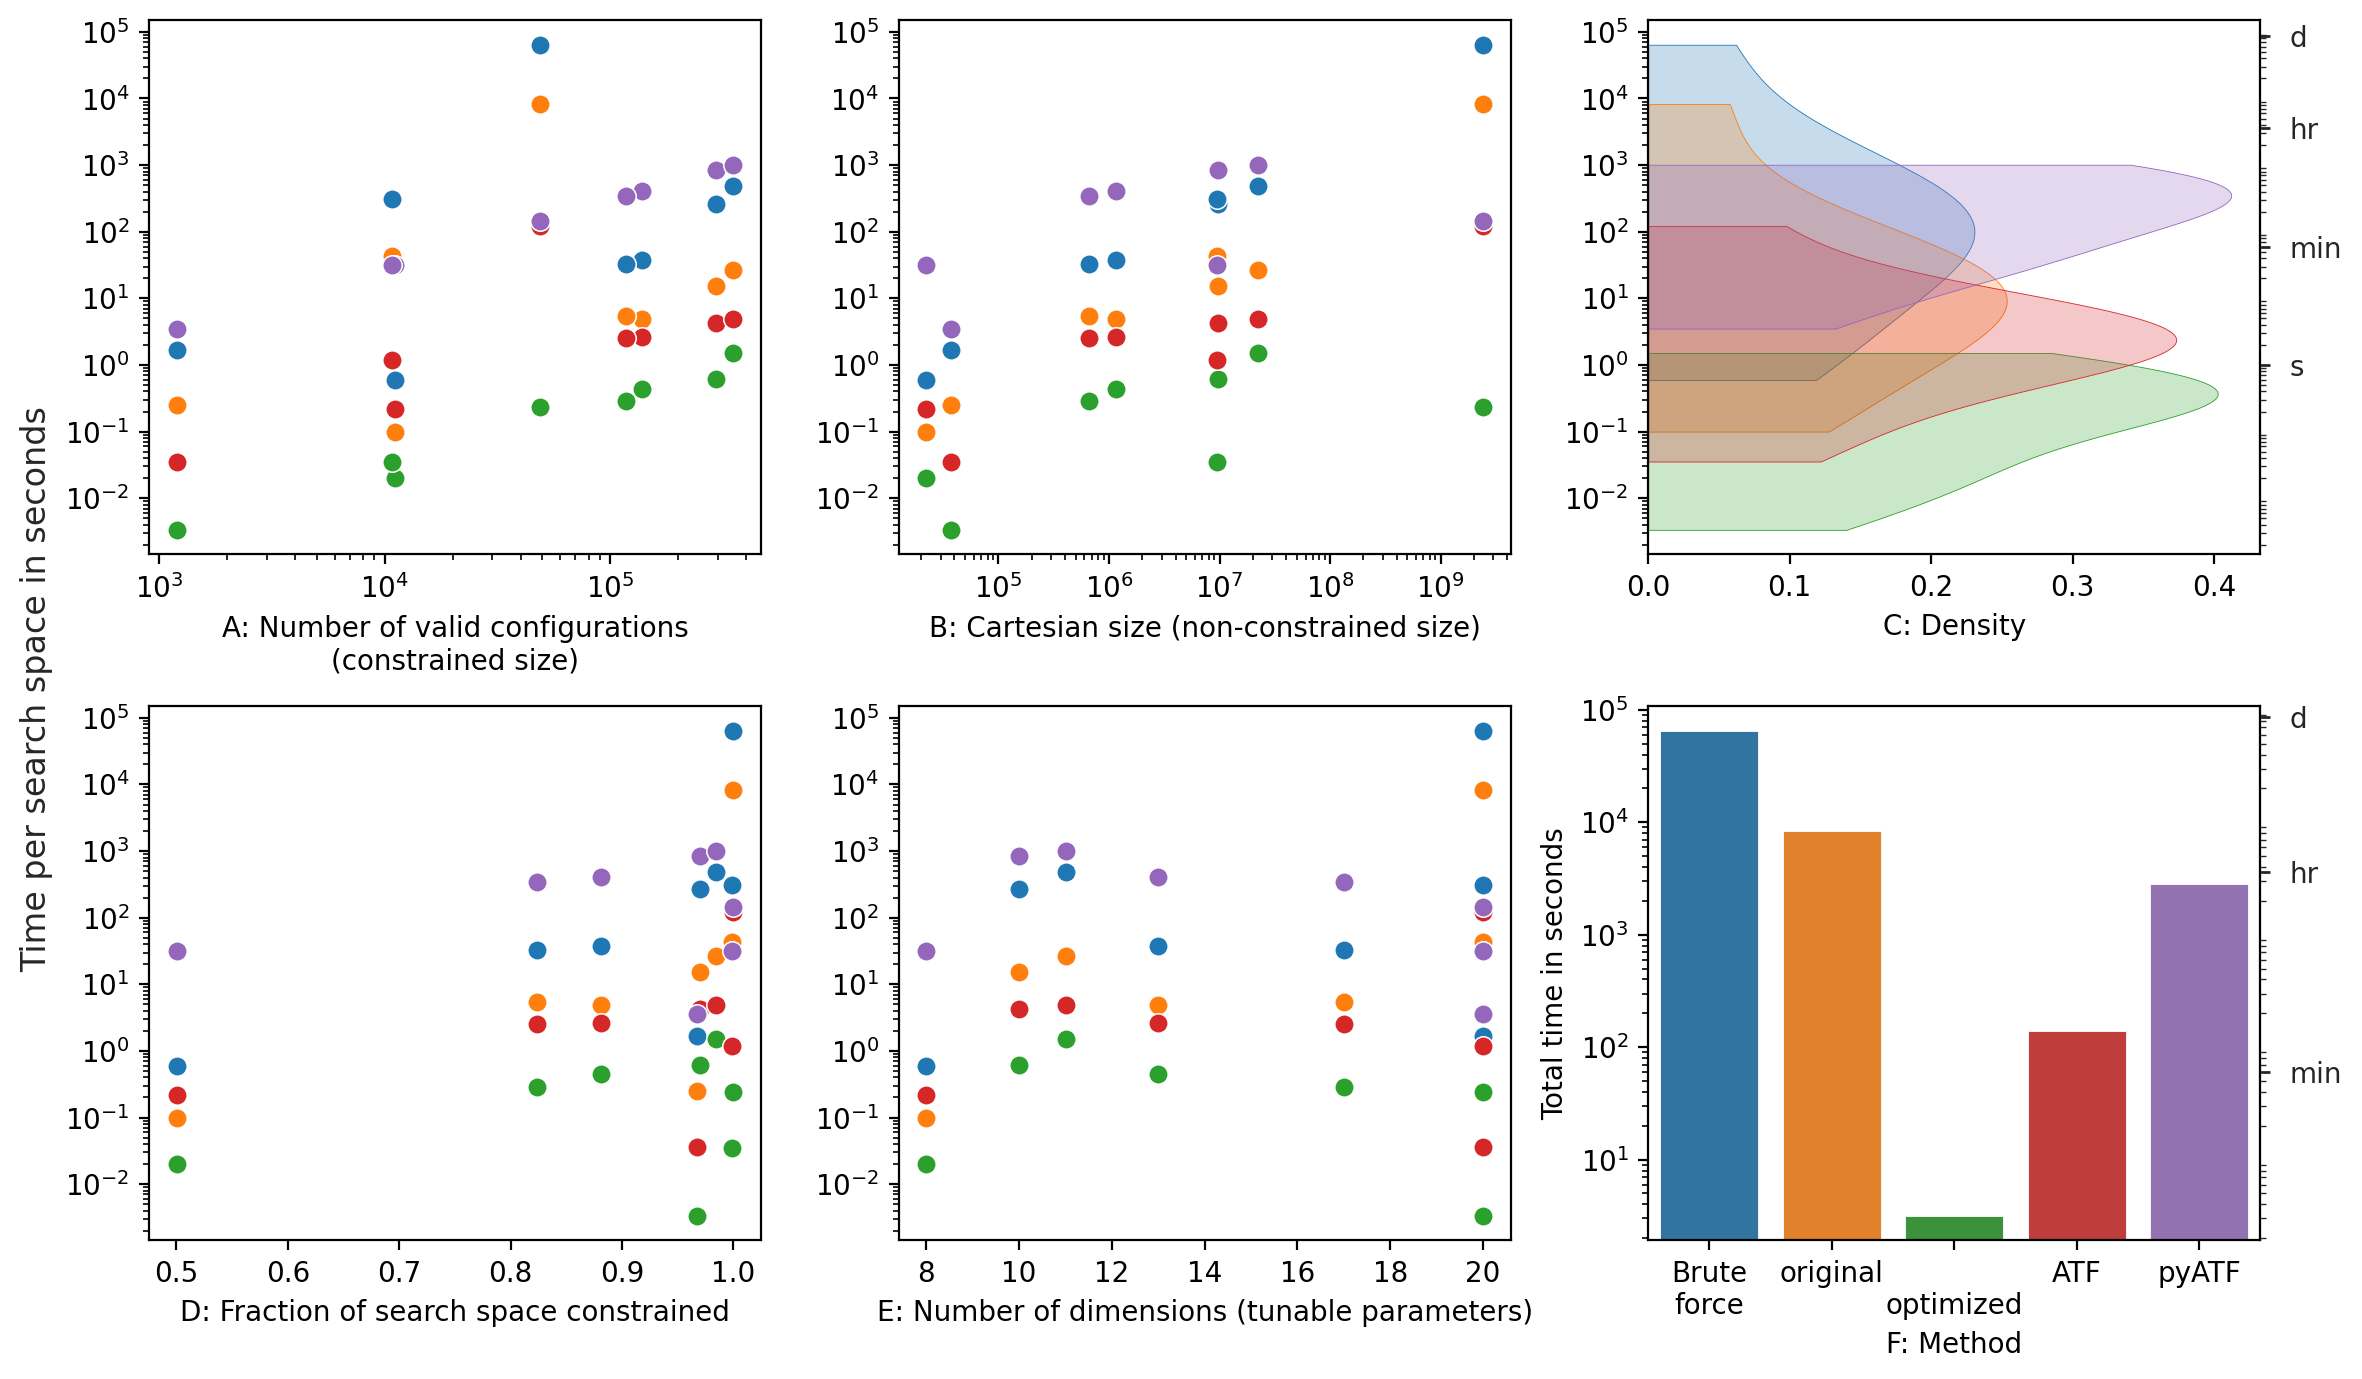
\includegraphics[width=1.0\textwidth]{ics25template/figures/searchspace_construction/results_realworld.png}
    \caption{Search space construction performance on real-world tests. Lower times are better. Colors correspond to \Cref{fig:results_realworld}F barplot methods.}
    \Description[Real-world search space construction performance]{Search space construction performance on real-world tests. Lower times are better.}
    \label{fig:results_realworld}
\end{figure*}

\subsubsection{Results} \label{subsubsec:evaluation_real-world_results}
\Cref{fig:results_realworld} presents the search space construction performance across the eight real-world benchmarks for five different constraint solver methods: \textit{brute force}, \textit{original}, \textit{optimized}, \textit{ATF}, and \textit{pyATF}. 
To determine the impact of the optimizations described in \cref{subsec:searchspace_construction_improvements}, the \textit{original} method denotes the use of vanilla \textit{python-constraint} before the optimizations, whereas our \textit{optimized} method includes the optimizations of \cref{subsec:searchspace_construction_improvements} as before in \cref{subsec:evaluation_synthetic}. 

\Cref{fig:results_realworld}A and \cref{fig:results_realworld}B illustrate the relationship between search space size and solver performance. In general, larger constrained search spaces (A) and Cartesian sizes (B) result in increased search times, particularly for the brute-force method. Our optimized solver consistently achieves the lowest execution times across all problem sizes, demonstrating its efficiency. ATF and pyATF show a similar trend but with higher execution times compared to our optimized solver, particularly for larger spaces. The original solver exhibits significantly higher execution times than our optimized version, though it performs better than the brute-force method.

\Cref{fig:results_realworld}C visualizes the distribution of execution times, providing an indication of the average performance and variability. 
Due to the substantially lower number of real-world search spaces compared to the synthetic search spaces, some observations made for \cref{fig:results_synthetic}C are obscured in \cref{fig:results_realworld}C, in particular the bimodality of the pyATF and ATF distributions. 
Nevertheless, it is interesting to observe that while the \textit{original} python-constraint method is one order of magnitude faster than the \textit{brute-force} method, both methods have very similar distributions. 
A clear trend emerges from this plot, where our optimized solver has the best performance and the least variability. 

In \cref{fig:results_realworld}D, the relation between how constrained a search space is and solver performance is displayed. 
In contrast to the synthetic tests in \cref{subsec:evaluation_synthetic}, the correlation between solver performance and the sparsity of the search space is not as clear. 
Nevertheless, \textit{ATF} and \textit{pyATF} performance again appears influenced by the sparsity, as for fraction $> 0.9$ \textit{ATF} performance is better than the \textit{original} solver, in contrast to $\leq 0.9$, where at fraction $\simeq 0.5$ even the unoptimized \textit{original} python-constraint outperforms \textit{ATF}. 

Similar to what is observed in \cref{subsec:evaluation_synthetic}, the number of tunable parameters displayed in \cref{fig:results_realworld}E do not appear to have as much of an impact on performance as the other plots discussed. 
Nevertheless, \cref{fig:results_realworld}E is useful to discern the individual search spaces based on the number of parameters. 
For instance, it can be noted that the performance difference between our optimized method and all other methods appears to be relatively stable, even for the ATF PRL search spaces detailed in \cref{tab:searchspaces_real_world_overview}, as can be discerned by the number of tunable parameters, where the three ATF search spaces have 20 tunable parameters.

Finally, \cref{fig:results_realworld}F summarizes the total time taken by each solver. 
The brute-force approach is the least performant, taking almost a full day to resolve the eight search spaces. 
Although the \textit{original} python-constraint solver is faster than brute force, our \textit{optimized} solver achieves a $\sim$2643x speedup over it, demonstrating the efficiency of our optimizations.
While ATF and pyATF achieve intermediate performance levels, the optimized solver considerably outperforms all others: our optimized method achieves a $\sim$20611x overall speedup over the brute-force method (3.16 seconds versus 65230.47 seconds), $\sim$44x over ATF, and $\sim$891x over pyATF. 
% As established in \cref{subsec:evaluation_synthetic}, these results confirm that solver performance is strongly influenced by the characteristics of the search space. 

Overall, it is noteworthy that our optimized solver consistently outperforms any alternative on all of the search spaces by a wide margin. 
These findings emphasize the advantages of our optimized solver in efficiently handling large and complex search spaces.

% Total speedup of method 'original' (8353.17 seconds) over 'Bruteforce' (65230.47 seconds): 7.8x
% Total speedup of method 'optimized' (3.16 seconds) over 'Bruteforce' (65230.47 seconds): 20610.7x
% Total speedup of method 'ATF' (137.83 seconds) over 'Bruteforce' (65230.47 seconds): 473.3x
% Total speedup of method 'pyATF' (2816.74 seconds) over 'Bruteforce' (65230.47 seconds): 23.2x


% Looking at the results of these tests in \cref{fig:results_realworld}, the performance difference is even more pronounced than in the synthetic tests: the optimized method achieves a $\sim$20611x overall speedup over the brute-force method (3.16 seconds versus 65230.47 seconds), is $\sim$44x faster than ATF, and $\sim$891x faster than pyATF. 
% It is interesting to note that the performance difference between our optimized method and all other methods appears to be relatively stable, even for the ATF PRL search spaces detailed in \cref{tab:searchspaces_real_world_overview}, as can be discerned by the number of tunable parameters in \cref{fig:results_realworld}E, where all ATF search spaces have 20 tunable parameters where the others do not.
% % On average over these real-world search spaces, our optimized method is three orders of magnitude faster than brute-forcing and one order of magnitude faster than the state-of-the-art in search space construction. 

% Finally, it is of interest to determine the impact of the optimizations. 
% In the results in \cref{fig:results_realworld}, the "\textit{original}" method denotes the use of \textit{python-constraint} before the optimizations described in \cref{subsec:searchspace_construction_improvements}, whereas the "\textit{optimized}" method includes the optimizations of \cref{subsec:searchspace_construction_improvements}. 
% While the \textit{original} method consistently outperforms \textit{bruteforce}, it does not outperform ATF and does not outperform PyATF on the ATF PRL search spaces. This is in contrast to the optimized method which consistently outperforms all other methods by a wide margin, confirming the efficacy of the optimizations. 
% % Total speedup of method 'Old' (8347.66 seconds) over 'Bruteforce' (65197.71 seconds): 7.8x
% % Total speedup of method 'New' (2.88 seconds) over 'Bruteforce' (65197.71 seconds): 22668.4x
% % Total speedup of method 'ATF' (135.3 seconds) over 'Bruteforce' (65197.71 seconds): 481.9x
% % Total speedup of method 'pyATF' (2474.65 seconds) over 'Bruteforce' (65197.71 seconds): 26.3x
